% Options for packages loaded elsewhere
\PassOptionsToPackage{unicode}{hyperref}
\PassOptionsToPackage{hyphens}{url}
%
\documentclass[
]{article}
\usepackage{lmodern}
\usepackage{amssymb,amsmath}
\usepackage{ifxetex,ifluatex}
\ifnum 0\ifxetex 1\fi\ifluatex 1\fi=0 % if pdftex
  \usepackage[T1]{fontenc}
  \usepackage[utf8]{inputenc}
  \usepackage{textcomp} % provide euro and other symbols
\else % if luatex or xetex
  \usepackage{unicode-math}
  \defaultfontfeatures{Scale=MatchLowercase}
  \defaultfontfeatures[\rmfamily]{Ligatures=TeX,Scale=1}
\fi
% Use upquote if available, for straight quotes in verbatim environments
\IfFileExists{upquote.sty}{\usepackage{upquote}}{}
\IfFileExists{microtype.sty}{% use microtype if available
  \usepackage[]{microtype}
  \UseMicrotypeSet[protrusion]{basicmath} % disable protrusion for tt fonts
}{}
\makeatletter
\@ifundefined{KOMAClassName}{% if non-KOMA class
  \IfFileExists{parskip.sty}{%
    \usepackage{parskip}
  }{% else
    \setlength{\parindent}{0pt}
    \setlength{\parskip}{6pt plus 2pt minus 1pt}}
}{% if KOMA class
  \KOMAoptions{parskip=half}}
\makeatother
\usepackage{xcolor}
\IfFileExists{xurl.sty}{\usepackage{xurl}}{} % add URL line breaks if available
\IfFileExists{bookmark.sty}{\usepackage{bookmark}}{\usepackage{hyperref}}
\hypersetup{
  pdftitle={Caso Euromotors},
  hidelinks,
  pdfcreator={LaTeX via pandoc}}
\urlstyle{same} % disable monospaced font for URLs
\usepackage[margin=1in]{geometry}
\usepackage{color}
\usepackage{fancyvrb}
\newcommand{\VerbBar}{|}
\newcommand{\VERB}{\Verb[commandchars=\\\{\}]}
\DefineVerbatimEnvironment{Highlighting}{Verbatim}{commandchars=\\\{\}}
% Add ',fontsize=\small' for more characters per line
\usepackage{framed}
\definecolor{shadecolor}{RGB}{248,248,248}
\newenvironment{Shaded}{\begin{snugshade}}{\end{snugshade}}
\newcommand{\AlertTok}[1]{\textcolor[rgb]{0.94,0.16,0.16}{#1}}
\newcommand{\AnnotationTok}[1]{\textcolor[rgb]{0.56,0.35,0.01}{\textbf{\textit{#1}}}}
\newcommand{\AttributeTok}[1]{\textcolor[rgb]{0.77,0.63,0.00}{#1}}
\newcommand{\BaseNTok}[1]{\textcolor[rgb]{0.00,0.00,0.81}{#1}}
\newcommand{\BuiltInTok}[1]{#1}
\newcommand{\CharTok}[1]{\textcolor[rgb]{0.31,0.60,0.02}{#1}}
\newcommand{\CommentTok}[1]{\textcolor[rgb]{0.56,0.35,0.01}{\textit{#1}}}
\newcommand{\CommentVarTok}[1]{\textcolor[rgb]{0.56,0.35,0.01}{\textbf{\textit{#1}}}}
\newcommand{\ConstantTok}[1]{\textcolor[rgb]{0.00,0.00,0.00}{#1}}
\newcommand{\ControlFlowTok}[1]{\textcolor[rgb]{0.13,0.29,0.53}{\textbf{#1}}}
\newcommand{\DataTypeTok}[1]{\textcolor[rgb]{0.13,0.29,0.53}{#1}}
\newcommand{\DecValTok}[1]{\textcolor[rgb]{0.00,0.00,0.81}{#1}}
\newcommand{\DocumentationTok}[1]{\textcolor[rgb]{0.56,0.35,0.01}{\textbf{\textit{#1}}}}
\newcommand{\ErrorTok}[1]{\textcolor[rgb]{0.64,0.00,0.00}{\textbf{#1}}}
\newcommand{\ExtensionTok}[1]{#1}
\newcommand{\FloatTok}[1]{\textcolor[rgb]{0.00,0.00,0.81}{#1}}
\newcommand{\FunctionTok}[1]{\textcolor[rgb]{0.00,0.00,0.00}{#1}}
\newcommand{\ImportTok}[1]{#1}
\newcommand{\InformationTok}[1]{\textcolor[rgb]{0.56,0.35,0.01}{\textbf{\textit{#1}}}}
\newcommand{\KeywordTok}[1]{\textcolor[rgb]{0.13,0.29,0.53}{\textbf{#1}}}
\newcommand{\NormalTok}[1]{#1}
\newcommand{\OperatorTok}[1]{\textcolor[rgb]{0.81,0.36,0.00}{\textbf{#1}}}
\newcommand{\OtherTok}[1]{\textcolor[rgb]{0.56,0.35,0.01}{#1}}
\newcommand{\PreprocessorTok}[1]{\textcolor[rgb]{0.56,0.35,0.01}{\textit{#1}}}
\newcommand{\RegionMarkerTok}[1]{#1}
\newcommand{\SpecialCharTok}[1]{\textcolor[rgb]{0.00,0.00,0.00}{#1}}
\newcommand{\SpecialStringTok}[1]{\textcolor[rgb]{0.31,0.60,0.02}{#1}}
\newcommand{\StringTok}[1]{\textcolor[rgb]{0.31,0.60,0.02}{#1}}
\newcommand{\VariableTok}[1]{\textcolor[rgb]{0.00,0.00,0.00}{#1}}
\newcommand{\VerbatimStringTok}[1]{\textcolor[rgb]{0.31,0.60,0.02}{#1}}
\newcommand{\WarningTok}[1]{\textcolor[rgb]{0.56,0.35,0.01}{\textbf{\textit{#1}}}}
\usepackage{graphicx,grffile}
\makeatletter
\def\maxwidth{\ifdim\Gin@nat@width>\linewidth\linewidth\else\Gin@nat@width\fi}
\def\maxheight{\ifdim\Gin@nat@height>\textheight\textheight\else\Gin@nat@height\fi}
\makeatother
% Scale images if necessary, so that they will not overflow the page
% margins by default, and it is still possible to overwrite the defaults
% using explicit options in \includegraphics[width, height, ...]{}
\setkeys{Gin}{width=\maxwidth,height=\maxheight,keepaspectratio}
% Set default figure placement to htbp
\makeatletter
\def\fps@figure{htbp}
\makeatother
\setlength{\emergencystretch}{3em} % prevent overfull lines
\providecommand{\tightlist}{%
  \setlength{\itemsep}{0pt}\setlength{\parskip}{0pt}}
\setcounter{secnumdepth}{-\maxdimen} % remove section numbering

\title{Caso Euromotors}
\author{}
\date{\vspace{-2.5em}}

\begin{document}
\maketitle

\#Header1 \{\#Descripción del problema\}

En este notebook les mostraré paso a paso el análisis del problema
propuesto. El objetivo de este problema es la resolución de las
siguientes incógnitas:

\begin{enumerate}
\def\labelenumi{\arabic{enumi}.}
\tightlist
\item
  ¿Cómo son los clientes de lujo para enfocar las estrategias de
  marketing?

  \begin{itemize}
  \tightlist
  \item
    Seleccionar las 10 variables más importantes del dataset
  \item
    ¿Son los precios similares a los de la realidad?
  \end{itemize}
\item
  ¿Cómo hacer la campaña de marketing más efectiva?

  \begin{itemize}
  \tightlist
  \item
    Seleccionar las variables más relevantes
  \item
    ¿De qué manera confirmaría que la propuesta es la adecuada?
  \end{itemize}
\end{enumerate}

\pagebreak

\begin{Shaded}
\begin{Highlighting}[]
\KeywordTok{library}\NormalTok{(DataExplorer) }\CommentTok{#para datos faltantes}
\end{Highlighting}
\end{Shaded}

\begin{verbatim}
## Warning: package 'DataExplorer' was built under R version 4.0.5
\end{verbatim}

\begin{Shaded}
\begin{Highlighting}[]
\KeywordTok{library}\NormalTok{(VIM) }\CommentTok{#para imputación de datos faltantes}
\end{Highlighting}
\end{Shaded}

\begin{verbatim}
## Warning: package 'VIM' was built under R version 4.0.4
\end{verbatim}

\begin{verbatim}
## Loading required package: colorspace
\end{verbatim}

\begin{verbatim}
## Warning: package 'colorspace' was built under R version 4.0.4
\end{verbatim}

\begin{verbatim}
## Loading required package: grid
\end{verbatim}

\begin{verbatim}
## VIM is ready to use.
\end{verbatim}

\begin{verbatim}
## Suggestions and bug-reports can be submitted at: https://github.com/statistikat/VIM/issues
\end{verbatim}

\begin{verbatim}
## 
## Attaching package: 'VIM'
\end{verbatim}

\begin{verbatim}
## The following object is masked from 'package:datasets':
## 
##     sleep
\end{verbatim}

\begin{Shaded}
\begin{Highlighting}[]
\KeywordTok{library}\NormalTok{(dplyr) }\CommentTok{#Para la manipulación de bases de datos}
\end{Highlighting}
\end{Shaded}

\begin{verbatim}
## Warning: package 'dplyr' was built under R version 4.0.5
\end{verbatim}

\begin{verbatim}
## 
## Attaching package: 'dplyr'
\end{verbatim}

\begin{verbatim}
## The following objects are masked from 'package:stats':
## 
##     filter, lag
\end{verbatim}

\begin{verbatim}
## The following objects are masked from 'package:base':
## 
##     intersect, setdiff, setequal, union
\end{verbatim}

\#\#\#Lectura de datos del CSV

\begin{Shaded}
\begin{Highlighting}[]
\NormalTok{db<-}\KeywordTok{read.csv}\NormalTok{(}\StringTok{"Base de datos caso práctico.csv"}\NormalTok{)}

\CommentTok{#View(db)}

\KeywordTok{dim}\NormalTok{(db)}
\end{Highlighting}
\end{Shaded}

\begin{verbatim}
## [1] 5000  124
\end{verbatim}

Son 5000 filas y 124 columnas

\#\#\#Busqueda de duplicados

\begin{Shaded}
\begin{Highlighting}[]
\NormalTok{n_occur<-}\KeywordTok{data.frame}\NormalTok{(}\KeywordTok{table}\NormalTok{(db}\OperatorTok{$}\NormalTok{custid))}
\NormalTok{n_occur[n_occur}\OperatorTok{$}\NormalTok{Freq}\OperatorTok{>}\DecValTok{1}\NormalTok{,]}
\end{Highlighting}
\end{Shaded}

\begin{verbatim}
## [1] Var1 Freq
## <0 rows> (or 0-length row.names)
\end{verbatim}

No hay customers duplicados

\#\#\#Cambio de variables categóricas a factors

\begin{Shaded}
\begin{Highlighting}[]
\NormalTok{db}\OperatorTok{$}\NormalTok{region<-}\KeywordTok{as.factor}\NormalTok{(db}\OperatorTok{$}\NormalTok{region)}
\NormalTok{db}\OperatorTok{$}\NormalTok{townsize<-}\KeywordTok{as.factor}\NormalTok{(db}\OperatorTok{$}\NormalTok{townsize)}
\NormalTok{db}\OperatorTok{$}\NormalTok{gender<-}\KeywordTok{as.factor}\NormalTok{(db}\OperatorTok{$}\NormalTok{gender)}
\NormalTok{db}\OperatorTok{$}\NormalTok{agecat<-}\KeywordTok{as.factor}\NormalTok{(db}\OperatorTok{$}\NormalTok{agecat)}
\NormalTok{db}\OperatorTok{$}\NormalTok{edcat<-}\KeywordTok{as.factor}\NormalTok{(db}\OperatorTok{$}\NormalTok{edcat)}
\NormalTok{db}\OperatorTok{$}\NormalTok{jobcat<-}\KeywordTok{as.factor}\NormalTok{(db}\OperatorTok{$}\NormalTok{jobcat)}
\NormalTok{db}\OperatorTok{$}\NormalTok{union<-}\KeywordTok{as.factor}\NormalTok{(db}\OperatorTok{$}\NormalTok{union)}
\NormalTok{db}\OperatorTok{$}\NormalTok{empcat<-}\KeywordTok{as.factor}\NormalTok{(db}\OperatorTok{$}\NormalTok{empcat)}
\NormalTok{db}\OperatorTok{$}\NormalTok{retire<-}\KeywordTok{as.factor}\NormalTok{(db}\OperatorTok{$}\NormalTok{retire)}
\NormalTok{db}\OperatorTok{$}\NormalTok{inccat<-}\KeywordTok{as.factor}\NormalTok{(db}\OperatorTok{$}\NormalTok{inccat)}
\NormalTok{db}\OperatorTok{$}\NormalTok{default<-}\KeywordTok{as.factor}\NormalTok{(db}\OperatorTok{$}\NormalTok{default)}
\NormalTok{db}\OperatorTok{$}\NormalTok{jobsat<-}\KeywordTok{as.factor}\NormalTok{(db}\OperatorTok{$}\NormalTok{jobsat)}
\NormalTok{db}\OperatorTok{$}\NormalTok{marital<-}\KeywordTok{as.factor}\NormalTok{(db}\OperatorTok{$}\NormalTok{marital)}
\NormalTok{db}\OperatorTok{$}\NormalTok{spousedcat<-}\KeywordTok{as.factor}\NormalTok{(db}\OperatorTok{$}\NormalTok{spousedcat)}
\NormalTok{db}\OperatorTok{$}\NormalTok{homeown<-}\KeywordTok{as.factor}\NormalTok{(db}\OperatorTok{$}\NormalTok{homeown)}
\NormalTok{db}\OperatorTok{$}\NormalTok{hometype<-}\KeywordTok{as.factor}\NormalTok{(db}\OperatorTok{$}\NormalTok{hometype)}
\NormalTok{db}\OperatorTok{$}\NormalTok{addresscat<-}\KeywordTok{as.factor}\NormalTok{(db}\OperatorTok{$}\NormalTok{addresscat)}
\NormalTok{db}\OperatorTok{$}\NormalTok{carown<-}\KeywordTok{as.factor}\NormalTok{(db}\OperatorTok{$}\NormalTok{carown)}
\NormalTok{db}\OperatorTok{$}\NormalTok{cartype<-}\KeywordTok{as.factor}\NormalTok{(db}\OperatorTok{$}\NormalTok{cartype)}
\NormalTok{db}\OperatorTok{$}\NormalTok{carcatvalue<-}\KeywordTok{as.factor}\NormalTok{(db}\OperatorTok{$}\NormalTok{carcatvalue)}
\NormalTok{db}\OperatorTok{$}\NormalTok{carbought<-}\KeywordTok{as.factor}\NormalTok{(db}\OperatorTok{$}\NormalTok{carbought)}
\NormalTok{db}\OperatorTok{$}\NormalTok{carbuy<-}\KeywordTok{as.factor}\NormalTok{(db}\OperatorTok{$}\NormalTok{carbuy)}
\NormalTok{db}\OperatorTok{$}\NormalTok{carcatvalue<-}\KeywordTok{as.factor}\NormalTok{(db}\OperatorTok{$}\NormalTok{carcatvalue)}
\NormalTok{db}\OperatorTok{$}\NormalTok{commute<-}\KeywordTok{as.factor}\NormalTok{(db}\OperatorTok{$}\NormalTok{commute)}
\NormalTok{db}\OperatorTok{$}\NormalTok{commutecat<-}\KeywordTok{as.factor}\NormalTok{(db}\OperatorTok{$}\NormalTok{commutecat)}
\NormalTok{db}\OperatorTok{$}\NormalTok{commutecar<-}\KeywordTok{as.factor}\NormalTok{(db}\OperatorTok{$}\NormalTok{commutecar)}
\NormalTok{db}\OperatorTok{$}\NormalTok{commuterail<-}\KeywordTok{as.factor}\NormalTok{(db}\OperatorTok{$}\NormalTok{commuterail)}
\NormalTok{db}\OperatorTok{$}\NormalTok{commutebus<-}\KeywordTok{as.factor}\NormalTok{(db}\OperatorTok{$}\NormalTok{commutebus)}
\NormalTok{db}\OperatorTok{$}\NormalTok{commutemotorcycle<-}\KeywordTok{as.factor}\NormalTok{(db}\OperatorTok{$}\NormalTok{commutemotorcycle)}
\NormalTok{db}\OperatorTok{$}\NormalTok{commutepublic<-}\KeywordTok{as.factor}\NormalTok{(db}\OperatorTok{$}\NormalTok{commutepublic)}
\NormalTok{db}\OperatorTok{$}\NormalTok{commutebike<-}\KeywordTok{as.factor}\NormalTok{(db}\OperatorTok{$}\NormalTok{commutebike)}
\NormalTok{db}\OperatorTok{$}\NormalTok{commutewalk<-}\KeywordTok{as.factor}\NormalTok{(db}\OperatorTok{$}\NormalTok{commutewalk)}
\NormalTok{db}\OperatorTok{$}\NormalTok{commutenonmotor<-}\KeywordTok{as.factor}\NormalTok{(db}\OperatorTok{$}\NormalTok{commutenonmotor)}
\NormalTok{db}\OperatorTok{$}\NormalTok{telecommute<-}\KeywordTok{as.factor}\NormalTok{(db}\OperatorTok{$}\NormalTok{telecommute)}
\NormalTok{db}\OperatorTok{$}\NormalTok{reason<-}\KeywordTok{as.factor}\NormalTok{(db}\OperatorTok{$}\NormalTok{reason)}
\NormalTok{db}\OperatorTok{$}\NormalTok{birthmonth<-}\KeywordTok{as.factor}\NormalTok{(db}\OperatorTok{$}\NormalTok{birthmonth)}
\NormalTok{db}\OperatorTok{$}\NormalTok{polview<-}\KeywordTok{as.factor}\NormalTok{(db}\OperatorTok{$}\NormalTok{polview)}
\NormalTok{db}\OperatorTok{$}\NormalTok{polparty<-}\KeywordTok{as.factor}\NormalTok{(db}\OperatorTok{$}\NormalTok{polparty)}
\NormalTok{db}\OperatorTok{$}\NormalTok{vote<-}\KeywordTok{as.factor}\NormalTok{(db}\OperatorTok{$}\NormalTok{vote)}
\NormalTok{db}\OperatorTok{$}\NormalTok{card<-}\KeywordTok{as.factor}\NormalTok{(db}\OperatorTok{$}\NormalTok{card)}
\NormalTok{db}\OperatorTok{$}\NormalTok{cardtype<-}\KeywordTok{as.factor}\NormalTok{(db}\OperatorTok{$}\NormalTok{cardtype)}
\NormalTok{db}\OperatorTok{$}\NormalTok{cardbenefit<-}\KeywordTok{as.factor}\NormalTok{(db}\OperatorTok{$}\NormalTok{cardbenefit)}
\NormalTok{db}\OperatorTok{$}\NormalTok{card2<-}\KeywordTok{as.factor}\NormalTok{(db}\OperatorTok{$}\NormalTok{card2)}
\NormalTok{db}\OperatorTok{$}\NormalTok{card2type<-}\KeywordTok{as.factor}\NormalTok{(db}\OperatorTok{$}\NormalTok{card2type)}
\NormalTok{db}\OperatorTok{$}\NormalTok{card2benefit<-}\KeywordTok{as.factor}\NormalTok{(db}\OperatorTok{$}\NormalTok{card2benefit)}
\NormalTok{db}\OperatorTok{$}\NormalTok{active<-}\KeywordTok{as.factor}\NormalTok{(db}\OperatorTok{$}\NormalTok{active)}
\NormalTok{db}\OperatorTok{$}\NormalTok{bfast<-}\KeywordTok{as.factor}\NormalTok{(db}\OperatorTok{$}\NormalTok{bfast)}
\NormalTok{db}\OperatorTok{$}\NormalTok{churn<-}\KeywordTok{as.factor}\NormalTok{(db}\OperatorTok{$}\NormalTok{churn)}
\NormalTok{db}\OperatorTok{$}\NormalTok{tollfree<-}\KeywordTok{as.factor}\NormalTok{(db}\OperatorTok{$}\NormalTok{tollfree)}
\NormalTok{db}\OperatorTok{$}\NormalTok{equip<-}\KeywordTok{as.factor}\NormalTok{(db}\OperatorTok{$}\NormalTok{equip)}
\NormalTok{db}\OperatorTok{$}\NormalTok{callcard<-}\KeywordTok{as.factor}\NormalTok{(db}\OperatorTok{$}\NormalTok{callcard)}
\NormalTok{db}\OperatorTok{$}\NormalTok{wireless<-}\KeywordTok{as.factor}\NormalTok{(db}\OperatorTok{$}\NormalTok{wireless)}
\NormalTok{db}\OperatorTok{$}\NormalTok{wiremon<-}\KeywordTok{as.factor}\NormalTok{(db}\OperatorTok{$}\NormalTok{wiremon)}
\NormalTok{db}\OperatorTok{$}\NormalTok{multline<-}\KeywordTok{as.factor}\NormalTok{(db}\OperatorTok{$}\NormalTok{multline)}
\NormalTok{db}\OperatorTok{$}\NormalTok{voice<-}\KeywordTok{as.factor}\NormalTok{(db}\OperatorTok{$}\NormalTok{voice)}
\NormalTok{db}\OperatorTok{$}\NormalTok{pager<-}\KeywordTok{as.factor}\NormalTok{(db}\OperatorTok{$}\NormalTok{pager)}
\NormalTok{db}\OperatorTok{$}\NormalTok{internet<-}\KeywordTok{as.factor}\NormalTok{(db}\OperatorTok{$}\NormalTok{internet)}
\NormalTok{db}\OperatorTok{$}\NormalTok{callid<-}\KeywordTok{as.factor}\NormalTok{(db}\OperatorTok{$}\NormalTok{callid)}
\NormalTok{db}\OperatorTok{$}\NormalTok{forward<-}\KeywordTok{as.factor}\NormalTok{(db}\OperatorTok{$}\NormalTok{forward)}
\NormalTok{db}\OperatorTok{$}\NormalTok{confer<-}\KeywordTok{as.factor}\NormalTok{(db}\OperatorTok{$}\NormalTok{confer)}
\NormalTok{db}\OperatorTok{$}\NormalTok{owntv<-}\KeywordTok{as.factor}\NormalTok{(db}\OperatorTok{$}\NormalTok{owntv)}
\NormalTok{db}\OperatorTok{$}\NormalTok{ownvcr<-}\KeywordTok{as.factor}\NormalTok{(db}\OperatorTok{$}\NormalTok{ownvcr)}
\NormalTok{db}\OperatorTok{$}\NormalTok{owndvd<-}\KeywordTok{as.factor}\NormalTok{(db}\OperatorTok{$}\NormalTok{owndvd)}
\NormalTok{db}\OperatorTok{$}\NormalTok{owncd<-}\KeywordTok{as.factor}\NormalTok{(db}\OperatorTok{$}\NormalTok{owncd)}
\NormalTok{db}\OperatorTok{$}\NormalTok{ownpda<-}\KeywordTok{as.factor}\NormalTok{(db}\OperatorTok{$}\NormalTok{ownpda)}
\NormalTok{db}\OperatorTok{$}\NormalTok{ownpc<-}\KeywordTok{as.factor}\NormalTok{(db}\OperatorTok{$}\NormalTok{ownpc)}
\NormalTok{db}\OperatorTok{$}\NormalTok{ownipod<-}\KeywordTok{as.factor}\NormalTok{(db}\OperatorTok{$}\NormalTok{ownipod)}
\NormalTok{db}\OperatorTok{$}\NormalTok{owngame<-}\KeywordTok{as.factor}\NormalTok{(db}\OperatorTok{$}\NormalTok{owngame)}
\NormalTok{db}\OperatorTok{$}\NormalTok{ownfax<-}\KeywordTok{as.factor}\NormalTok{(db}\OperatorTok{$}\NormalTok{ownfax)}
\NormalTok{db}\OperatorTok{$}\NormalTok{news<-}\KeywordTok{as.factor}\NormalTok{(db}\OperatorTok{$}\NormalTok{news)}
\NormalTok{db}\OperatorTok{$}\NormalTok{response_}\DecValTok{01}\NormalTok{<-}\KeywordTok{as.factor}\NormalTok{(db}\OperatorTok{$}\NormalTok{response_}\DecValTok{01}\NormalTok{)}
\NormalTok{db}\OperatorTok{$}\NormalTok{response_}\DecValTok{02}\NormalTok{<-}\KeywordTok{as.factor}\NormalTok{(db}\OperatorTok{$}\NormalTok{response_}\DecValTok{02}\NormalTok{)}
\NormalTok{db}\OperatorTok{$}\NormalTok{response_}\DecValTok{03}\NormalTok{<-}\KeywordTok{as.factor}\NormalTok{(db}\OperatorTok{$}\NormalTok{response_}\DecValTok{03}\NormalTok{)}
\end{Highlighting}
\end{Shaded}

Ahora veamos que columnas tienen una alta cantidad de valores nulos

\begin{Shaded}
\begin{Highlighting}[]
\KeywordTok{plot_missing}\NormalTok{(db,}\DataTypeTok{missing_only =} \OtherTok{TRUE}\NormalTok{)}
\end{Highlighting}
\end{Shaded}

\includegraphics{Caso-Euromotors_files/figure-latex/unnamed-chunk-6-1.pdf}

Se pasan a eliminar las columans con datos faltantes mayores al 20\% (5
columnas)

\begin{Shaded}
\begin{Highlighting}[]
\NormalTok{db<-db[, }\KeywordTok{colMeans}\NormalTok{(}\KeywordTok{is.na}\NormalTok{(db)) }\OperatorTok{<=}\StringTok{ }\FloatTok{.2}\NormalTok{]}
\KeywordTok{dim}\NormalTok{(db)}
\end{Highlighting}
\end{Shaded}

\begin{verbatim}
## [1] 5000  119
\end{verbatim}

A continuación podemos ver las columnas que quedan con datos faltantes

\begin{Shaded}
\begin{Highlighting}[]
\KeywordTok{plot_missing}\NormalTok{(db,}\DataTypeTok{missing_only =} \OtherTok{TRUE}\NormalTok{)}
\end{Highlighting}
\end{Shaded}

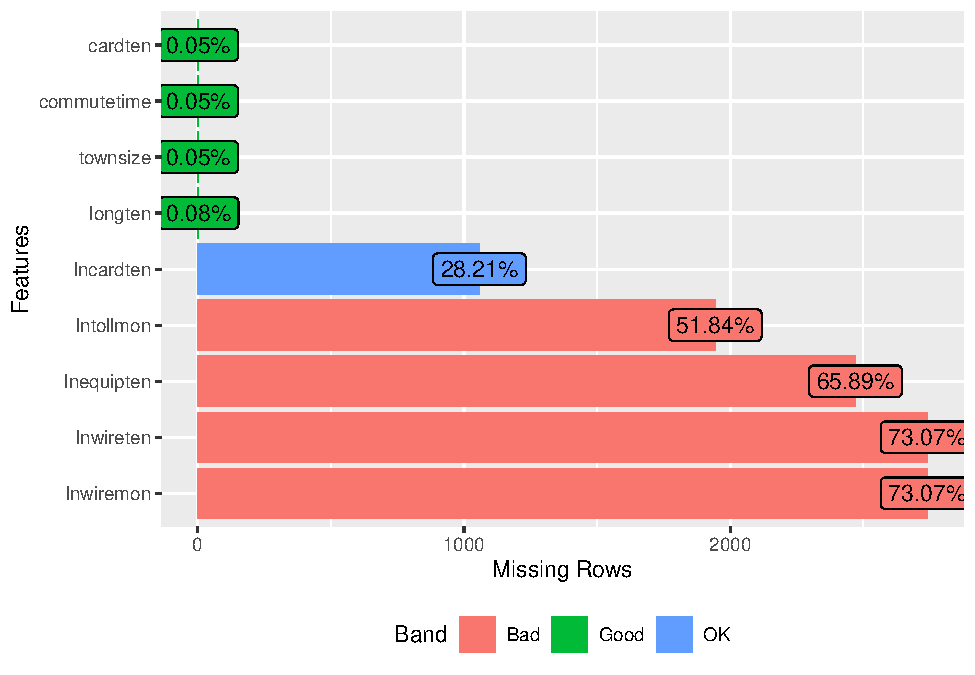
\includegraphics{Caso-Euromotors_files/figure-latex/unnamed-chunk-8-1.pdf}
Ahora, se pasará a imputar estas columnas

\begin{Shaded}
\begin{Highlighting}[]
\NormalTok{db<-}\KeywordTok{kNN}\NormalTok{(db)}
\NormalTok{db<-db}\OperatorTok\KeywordTok{select}\NormalTok{(}\OperatorTok{-}\KeywordTok{ends_with}\NormalTok{(}\StringTok{"_imp"}\NormalTok{)) }\CommentTok{#Para eliminar las adicionales que se generan en la imputación}
\end{Highlighting}
\end{Shaded}

Finalmente, guardamos una copia de seguridad de los datos limpios

\begin{Shaded}
\begin{Highlighting}[]
\KeywordTok{write.csv}\NormalTok{(db,}\StringTok{"db_clean.csv"}\NormalTok{)}
\end{Highlighting}
\end{Shaded}

\end{document}
